%
% $Id: slides.tex 4228 2010-11-24 17:55:12Z pcoca $
%
%
% Compilar a .pdf con LaTeX (pdflatex)
% Es necesario instalar Beamer (paquete latex-beamer en Debian)
%

%
% Gráficos:
% Los gráficos pueden suministrarse en PNG, JPG, TIF, PDF, MPS
% Los EPS deben convertirse a PDF (usar epstopdf)
%

\documentclass{beamer}
\usetheme{Warsaw}
\usebackgroundtemplate{
\includegraphics[width=\paperwidth]{format/libresoft-bg.png}}
\usepackage[spanish]{babel}
\usepackage[utf8]{inputenc}
\usepackage{graphics}
\usepackage{amssymb} % Simbolos matematicos
\usepackage{url}

%\definecolor{libresoftgreen}{RGB}{162,190,43}
%\definecolor{libresoftblue}{RGB}{0,98,143}

%\setbeamercolor{titlelike}{bg=libresoftgreen}

%% Metadatos del PDF.
\hypersetup{
  pdftitle={OpenBRR},
  pdfauthor={G. Robles, F. Ortega, D. Izquierdo, P. Coca},
  pdfcreator={GSyC/Libresoft},
  pdfproducer=PDFLaTeX,
  pdfsubject={nn},
}
%%


\AtBeginSection[]
{
  \begin{frame}<presentation>
    \frametitle{Index}
    \tableofcontents[current]
  \end{frame}
}


\begin{document}

\title{QSOS}
\subtitle{OpenBRR}
\institute{\\pcoca@libresoft.es\\
GSyC/Libresoft}
\author{Gregorio Robles, Felipe Ortega, Daniel Izquierdo, Pedro Coca}
\date{\today}

\frame{
\maketitle
\begin{center}

\includegraphics[width=6cm]{format/gsyc-urjc}
\end{center}
}


% Si el titulo o el autor se quieren acortar para los pies de página
% se pueden redefinir aquí:
%\title{Titulo corto}
%\author{Autores abreviado}


%% LICENCIA DE REDISTRIBUCION DE LAS TRANSPAS
\frame{
~
\vspace{4cm}

\begin{flushright}
{\tiny
(cc) 2010 Gregorio Robles, Felipe Ortega, Daniel Izquierdo, Pedro Coca. \\
Some rights reserved. This document is distributed under the Creative \\
            Commons Attribution-ShareAlike 3.0 licence, available in \\
            http://creativecommons.org/licenses/by-sa/3.0/

%  Este documento (o uno muy similar) está disponible en \\
%  \url{http://gsyc.escet.urjc.es/~jjamor/}
}
\end{flushright}
}
%%

%%%%%%
%Transpas separadas por \begin{frame}
%%%%%%%%%%%%%%%%%%%%%%%%\end{frame}


\section{OpenBRR}


\begin{frame}
\frametitle{Introduction}

\begin{itemize}
\item Evaluating software is a critical task for IT managers responsible for the selection of software components
\item There is currently no easy, effective and trustworthy element for assessing free software
\item The Business Readiness Rating OpenBRR is being proposed as an open and standard framework to quickly make informed and educated decisions on free software
\item Lead by the CarnegieMellon West University, Spike Source, Intel and O'Reilly's Code Zoo
\end{itemize}

\end{frame}

\begin{frame}
\frametitle{The challenge}

Users and potential adopters of free software face following challenges:

\begin{itemize}
\item Selection
\item Support
\item Longevity
\item Volatility
\item Low quality
\end{itemize}

\end{frame}



\begin{frame}
\frametitle{Before Standard and Open Model}


\begin{center}
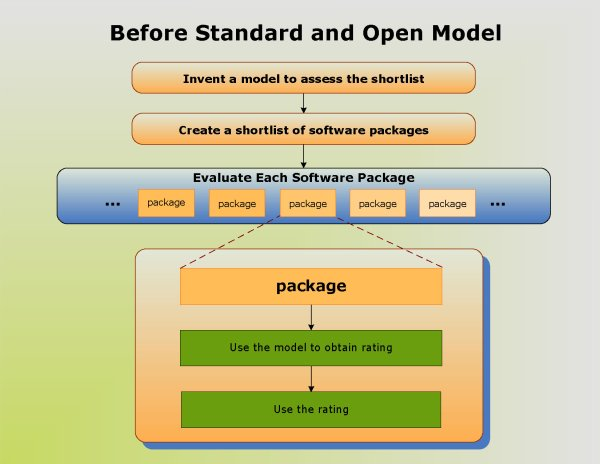
\includegraphics[width=8cm]{figs/Before_standard_and_open_model.jpg}
\end{center}

\end{frame}

\begin{frame}

\frametitle{Looking for an Open and Standard Model}

Characteristics of the model (CSAC)

\begin{itemize}
\item Complete (every prominent characteristic)
\item Simple
\item Adaptable
\item Consistent
\end{itemize}

Allows to share assessment results, promotes trust.

\end{frame}



\begin{frame}
\frametitle{After a Standard and Open Model}

\begin{center}
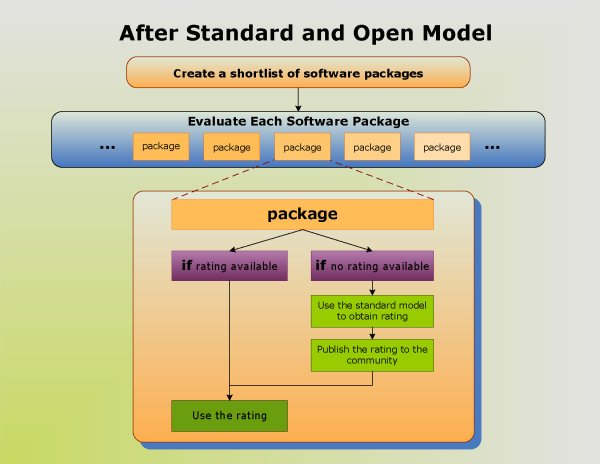
\includegraphics[width=8cm]{figs/After_standard_and_open_model.jpg}
\end{center}

\end{frame}



\begin{frame}
\frametitle{The Four Phases of Software Assessment}

\begin{center}
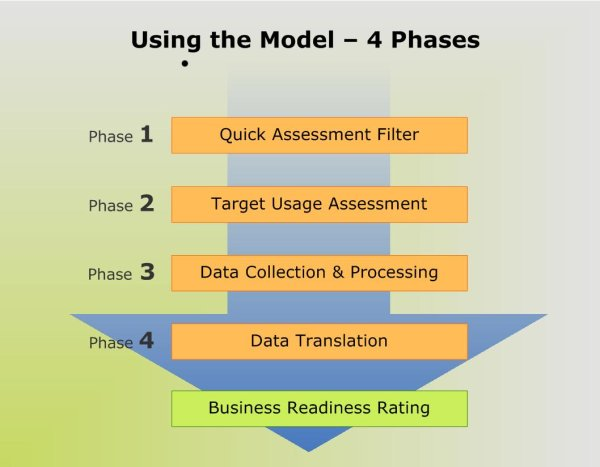
\includegraphics[width=8cm]{figs/Using_the_Model_-_4_Phases.jpg}
\end{center}

\end{frame}


\begin{frame}

\frametitle{Intial Filtering}

Quick Assessment Phase:

\begin{itemize}
\item  What is the licensing/legal situation of the software?
\item  Does it comply with standards?
\item  Are there referenceable adopters or users for it?
\item  Is a supporting or stable organization associated with the development efforts?
\item  What is its implementation language?
\item  Does it support internationalization and localization in your desired language?
\item  Are there third-party reviews of the software?
\item  Have books been published about the software?
\item  Is it being followed by industry analysts, such as Gartner or IDC?
\end{itemize}


\end{frame}


\begin{frame}

\frametitle{Metrics and Categories}

\begin{itemize}
\item Functionality
\item Usability
\item Quality
\item Security
\item Performance
\item Scalability
\item Architecture
\item Support
\item Documentation
\item Adoption
\item Community
\item Professionalism
\end{itemize}

\end{frame}



\begin{frame}
\frametitle{OpenBRR in detail: Weightings}

\begin{center}
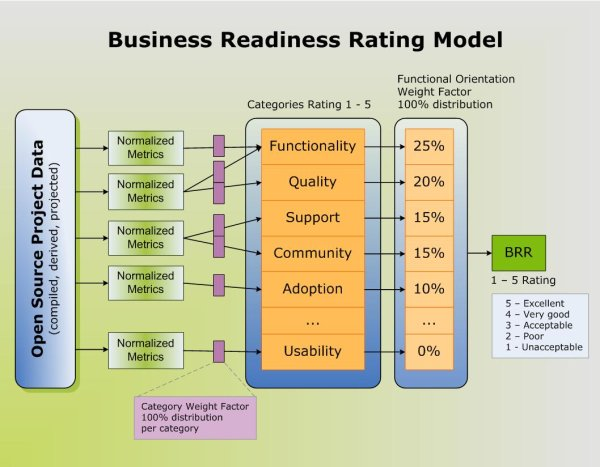
\includegraphics[width=8cm]{figs/Business_Ready_Rating_Model.jpg}
\end{center}

\end{frame}


%%%%%%%%%%%%%%%%%%%%%%%%%%%%%%%%%%%%%%%%%%%%%%%%%%%%%%%%%%%%%%

\end{document}
